\begin{figure}[t]
\centering
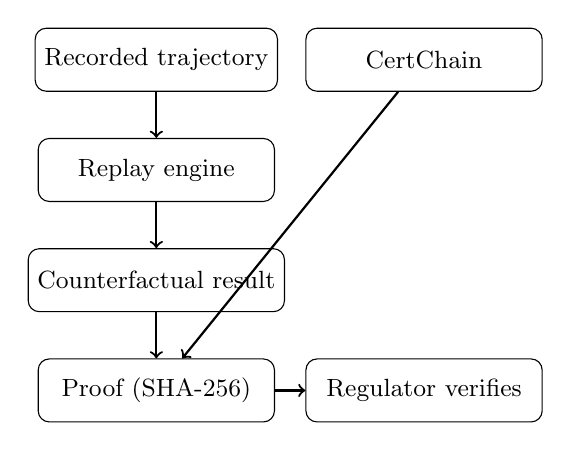
\begin{tikzpicture}[
    node distance=1.4cm,
    every node/.style={font=\small, draw, rectangle, rounded corners,
                        minimum width=3cm, minimum height=0.8cm, align=center}
]
\node (traj) {Recorded trajectory};
\node (chain) [right of=traj, xshift=2cm] {CertChain};
\node (replay) [below of=traj] {Replay engine};
\node (result) [below of=replay] {Counterfactual result};
\node (proof) [below of=result] {Proof (SHA-256)};
\node (verify) [right of=proof, xshift=2cm] {Regulator verifies};
\draw[->, thick] (traj) -- (replay);
\draw[->, thick] (replay) -- (result);
\draw[->, thick] (result) -- (proof);
\draw[->, thick] (chain) -- (proof);
\draw[->, thick] (proof) -- (verify);
\end{tikzpicture}
\caption{CSR architecture. The trajectory is replayed under modified
conditions; the result is bound to the original chain via SHA-256.}
\label{fig:csr-arch}
\end{figure}
